\documentclass[11pt, oneside]{article} 
\usepackage{geometry}
\geometry{letterpaper} 
\usepackage{graphicx}
	
\usepackage{amssymb}
\usepackage{amsmath}
\usepackage{parskip}
\usepackage{color}
\usepackage{hyperref}

\graphicspath{{/Users/telliott_admin/Tex/png/}}
% \begin{center} \includegraphics [scale=0.4] {gauss3.png} \end{center}

\title{Fermat and Euler's Theorems}
\date{}

\begin{document}
\maketitle
\Large

\subsection*{theorem}
Fermat's Theorem is often called Fermat's "little" Theorem to distinguish it from his more famous "Last" theorem.

The theorem says that for any prime number $p$ and any integer $1 < a < n$ 
\[ a^p  \text{ mod } p = a \]
Two equivalent statements are
\[ a^{p-1} \text{ mod } p = 1 \]
\[ (a^p - a)  \text{ mod } p = 0 \]

The second statement is what we use in analyzing the RSA method, and the third is used in the combinatorial proof of the theorem.

Examples:
\begin{verbatim}
2^3 mod 3 =   8 mod 3 = 2
2^5 mod 5 =  32 mod 5 = 2
3^5 mod 5 = 243 mod 5 = 3
\end{verbatim}

Consider $p=7$
\begin{verbatim}
1^6       1 mod 7 = 1
2^6 =    64 mod 7 = 1
3^6 =   729 mod 7 = 1
4^6 =  4096 mod 7 = 1
5^6 = 15625 mod 7 = 1
6^6 = 46656 mod 7 = 1
\end{verbatim}
Here is a table from Laws of Cryptography  for $p = 13$, which computes such powers more efficiently (by computing mod $p$ at each step).
\begin{center} 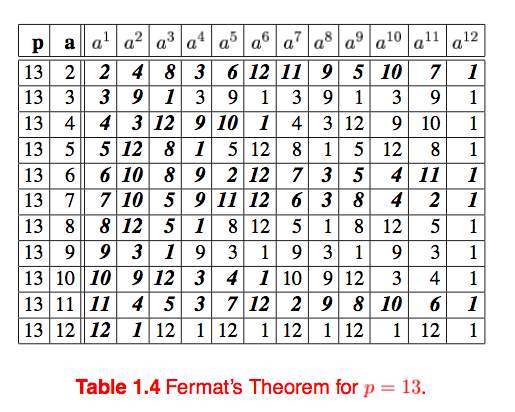
\includegraphics [scale=0.65] {Fermat13.png} \end{center}

\url{www.cs.utsa.edu/~wagner/lawsbookcolor/laws.pdf}

Let's do the calculation for $a = 7, p = 13$:
\begin{verbatim}
7**1  =               7
7**2  = 49 - 3(13) = 10
7**3  = 70 - 5(13) =  5
7**4  = 35 - 2(13) =  9
7**5  = 63 - 4(13) = 11
7**6  = 77 - 5(13) = 12
7**7  = 84 - 6(13) =  6
7**8  = 42 - 3(13) =  3
7**9  = 21 - 1(13) =  8
7**10 = 56 - 4(13) =  4
7**11 = 28 - 2(13) =  2
7**12 = 14 - 1(13) =  1
\end{verbatim}

As the theorem says, we cycle around to $7^{12}$ mod $13 = 1$.  The number $7$ is called a \emph{generator} because its powers generate all the values in the field $Z_{13}$. 

$2, 6$ and $11$ are also generators for $Z_{13}$.

Other values for $a$ have shorter repeats (2, 3, 4 or 6 long).  The lengths of such runs must be divisors of 12 so that they can cycle around after 12 rounds.

\subsection*{proofs of Fermat's Theorem}

Fermat didn't actually prove his theorem.  Euler proved something more general, the theorem we introduce below, and Fermat is a specific case of that.

There is a beautiful combinatorial proof called the "necklace proof".  Here is a write-up:

\small
\url{http://scienceblogs.com/evolutionblog/2010/04/15/a-combinatorial-proof-of-ferma/}
\Large

\subsection*{combinatorial proof}

We construct a necklace of $p$ beads, choosing from $a$ different colors.  We start by threading beads onto a linear piece of string.

Since we can choose any one of $a$ colors, $p$ times, there are $a^p$ possible sequences.

However, we wish to exclude arrangements where all the beads have the same color  There are $a$ of these and so the number of arrangements is $a^p - a$.

Now, join the ends of the string.  As a cycle, each shifted sequence becomes indistinguishable from the others.  There are $p$ such cyclic shifts for each linear arrangement.  For example, any cyclic permutation of $ABCBAAC$ looks the same:

\begin{center} 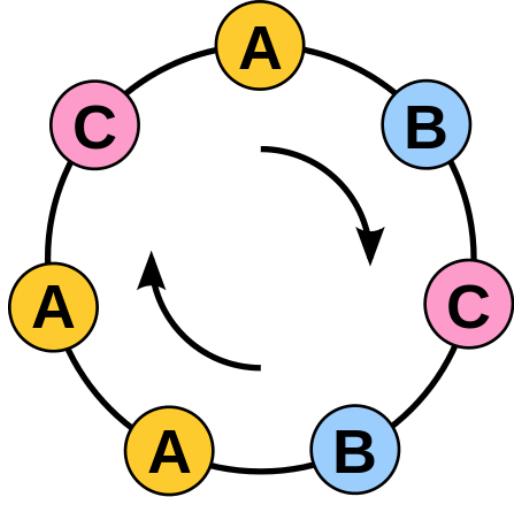
\includegraphics [scale=0.3] {necklace.png} \end{center}

Therefore, the total number of arrangements is reduced by a factor of $p$.
\[ n = \frac{a^p - a}{p} \]

The key observation is that $n$, the number of different arrangements, is clearly an integer.  So we have that
\[ a^p - a = np \]
If we take the modulus of both sides (mod $p$) we have the result we seek.
\[ (a^p - a)  \text{ mod } p = 0 \]

$\square$

\subsection*{proof by induction}

This proof is just as simple.  We claim that
\[ a^p  \text{ mod } p = a \]
The base case is $1^p$ mod $p = 1$, which is obviously true.  

The binomial theorem gives this expansion for 
\[  (a+1)^p = a^p + \binom{p}{1} a^{p-1} + + \binom{p}{2} a^{p-2} + \dots + \binom{p}{p-1} a + 1  \]
All terms on the right-hand side except the first and last have $p$ as a factor, so mod $p$ each is just zero.  We have
\[  (a+1)^p \text{ mod } p = (a^p + 1)  \text{ mod } p \]
For the inductive step, we may assume that $a^p  \text{ mod } p = a$, so this becomes
\[ (a+1)^p \text{ mod } p= (a + 1) \text{ mod } p \]
which completes the proof.

$\square$

\subsection*{consequence}
A consequence of this theorem is that the sequence $a^1, \ a^2, \ a^3 \dots a^{p-1}$ repeats, so the sequence $a^{p}, a^{p+1} \dots a^{2p - 1}$ consists of exactly the same values.

As the source says:

\textbf{Because $a$  to a power $x$ mod $p$ always starts repeating after the power reaches $p-1$, one can reduce the power mod $p-1$ and still get the same answer."}

Thus no matter how big the power $x$ in
\[ a^x \text{ mod } p \]
then let
\[ y = x \text{ mod } (p-1) \]
and so
\[ a^x \text{ mod } p = a^{y} \text{ mod } p \]
For example, mod $13$:
\[ a^{29} \text{ mod } 13 = a^{29 \text{ mod } 12} \text{ mod } 13 \]
\[ = a^5  \text{ mod } 13 \]

Of course, it is possible that the sequence may repeat even more quickly, as we saw with the table above.

\subsection*{Euler}
Euler's totient function $\phi(n)$ is defined like so:
\[ \phi(n) = n \ \prod \ (1 - \frac{1}{p_i}) \]
where the $p_i$ are the prime factors of $n$.  In number theory, $\phi$ gives the count of the positive integers up to a given integer $n$ that are relatively prime to $n$, that are not divisors of $n$.

\subsection*{theorem}
Relevant to our study of cryptography, Euler's Theorem says that for an integer $a < p$ (not equal to $1$):
\[ a^{\phi(n)} \text{ mod } n = 1 \]
If $n$ is prime this reduces to 
\[ \phi(n) = n \ \prod (1 - \frac{1}{n}) =  n(1 -  \frac{1}{n}) = n - 1 \]
and so
\[ a^{n-1} \text{ mod } n = 1 \]
Fermat's Theorem is a special case of Euler's Theorem, when $n$ is prime.

We skip the proof.  See

\small
\url{https://artofproblemsolving.com/wiki/index.php?title=Euler%27s_Totient_Theorem}
\Large

\subsection*{cryptography}
Here we are particularly interested in the situation where $n$ has two large prime factors $p$ and $q$ and then:
\[ \phi(n) = pq \ (1 - \frac{1}{p}) (1 - \frac{1}{q}) = (p - 1)(q - 1)  \]

Furthermore, we have defined encryption followed by decryption in public key cryptography as $m^{ed} \text{ mod } n = m$.  We would like to show that this follows as a consequence of our definitions.  

From now on, we write $\phi$ for $\phi(n)$.  Recall that $d$ is defined to be the multiplicative inverse of $e$ mod $\phi$. 

Write out what's given:
\[ \phi = (p - 1)(q - 1) \]
\[ m^{\phi} \text{ mod } n = 1 \]
\[ ed  \text{ mod } \phi = 1 \]
Our chained encryption/decryption is $(m^{e})^{d}$ mod $n$  or:
\[ m^{ed} \text{ mod } n \]

My source says:  "similar to Fermat's Theorem, arithmetic in the exponent is taken mod $\phi$."  

The idea is that since  
\[ m^{\phi} \text{ mod } n = 1 \]

if we are computing any \emph{other} power of $m$, say $ed$, we need only compute to the power of $ed$ mod $\phi$, because beyond that, the sequence just repeats.

We saw the repetition for Fermat's Theorem;  it happens here as well, even though $n$ is not prime.  However, it is required that $m$ be coprime to $n$.  

As a counter-example, take $n = 6 = 2*3$.  Then $\phi = 2$.  

Now, $5^2 = 25 = 1$ mod $6$. 

 But $4^2 = 16$ mod $6 = 4$.  Thus, $4$ to \emph{any} power mod $6$ is $4$!.  The difference is that $4$ is not coprime to $6$, but $5$ is.

For the big example, we have $m$  to the power $ed$ and then mod $pq$, and we reduce the power $ed$ mod $\phi$ since $\phi = (p-1)(q-1)$.

(Assuming $m$ has no common divisors with $n$):
\[ m^{ed} \text{ mod } n = m^{ed} \text{ mod } pq \]
\[ = m^{ed \text{ mod } \phi} \text{ mod } pq \]
But of course $ed \text{ mod } \phi = 1$ so this is just $m$.

Furthermore, $m^{ed} = m^{de}$, hence the ability to encrypt first with the private key and then decrypt with the public one.

\end{document}  